% don't remove the following lines, and edit the definition of \main if needed
\documentclass[../report.tex]{subfiles}
\providecommand{\main}{..}
\IfEq{\jobname}{\currfilebase}{\AtEndDocument{\biblio}}{}
\IfEq{\jobname}{\currfilebase}{%file for shortcuts

\newcommand{\nch}{\ensuremath{N_{\mathrm {ch}}\xspace}}
\newcommand{\dNdeta}{\mathrm{d}N_\mathrm{ch}/\mathrm{d}\eta}
}{}
% until here

\newcommand{\mlna}{\langle \ln\!A \rangle}
\newcommand{\nmu}{N_\mu}
\newcommand{\lnnmu}{\ln\!\nmu}
\newcommand{\xmax}{X_\text{max}}
\newcommand{\nmult}{N_\text{mult}}
\newcommand{\tocite}{{\bf REF}}
\newcommand{\si}[1]{\ensuremath{\text{#1}}}
\newcommand{\SI}[2]{\ensuremath{#1\,\si{#2}}}

\begin{document}

\section{Beyond...}

\subsection{Proton-oxygen collisions for cosmic ray research}
\label{sec:pOcosmic}

\begin{figure}
\includegraphics[width=0.5\textwidth,trim=5 -5 20 0]{\main/beyond/fig/lna_uncertainty.pdf}
\includegraphics[width=0.5\textwidth,trim=-20 0 30 0]{\main/beyond/fig/epos_mod.pdf}
\caption{\emph{Left panel:} Mass composition of cosmic rays quantified by $\mlna$ as a function of cosmic ray energy $E$. See Ref.~\cite{kampert_cr_review} for references to data (bands) and model predictions (markers and lines), and the text for a discussion. \emph{Right panel:} Projected impact of measurements of hadron multiplicity $\nmult$ and the energy fraction $\alpha$ which goes into neutral pions in pp collisions at \SI{13}{TeV} on EPOS-LHC predictions for mean $\xmax$ and $\lnnmu$ in $10^{19}$\,\si{eV} air showers, compared to Auger data~\cite{Aab:2014pza}. The model lines represent all values that can be obtained for any mixture of cosmic nuclei from proton to iron. The dashed and dotted lines represent modifications of $\nmult$ and $\alpha$ in steps of $\pm$10\% from their nominal values.}
\label{fig:cosmic_rays}
\end{figure}

The recent coincident observations of gamma rays and neutrinos from the flaring blazar TXS 0506+056 confirmed that active galactic nuclei produce high-energy cosmic rays~\cite{IceCube:2018dnn}. This is a long awaited finding demonstrates that sources of cosmic rays are linked to the most violent places in our universe. Measurements of cosmic rays contribute to the understanding of the high-energy universe. Since cosmic rays are charged and bent onto chaotic paths by magnetic fields in space, their arrival directions are highly isotropic, but their mass composition contains a unique imprint from the source physics.

Cosmic rays are nuclei from proton to iron, with a negligible fraction of heavier elements. The mass composition of cosmic rays in a given energy interval is characteristic for different source scenarios. This is shown in Fig.~\ref{fig:cosmic_rays}, left-hand-side, where the mean-logarithmic-mass $\mlna$ of cosmic rays is shown for several source scenarios (lines and markers). The model predictions are compared to a compilation of experimental data. Above $10^{15}$\,\si{eV}, $\mlna$ can only be indirectly inferred from extensive air showers, huge secondary particle cascades produced by collisions between cosmic ray and nuclei in the atmosphere. The two leading observables to infer $\mlna$ are the depth $\xmax$ of the shower maximum in the atmosphere (yellow band in Fig.~\ref{fig:cosmic_rays}), and the number $\nmu$ of muons produced in the shower (green band in Fig.~\ref{fig:cosmic_rays}). The width of those bands has two main contributions: the experimental uncertainties, and the model uncertainties inherent in converting the air shower observables into $\mlna$.

Leading experiments achieve an experimental uncertainty of 10 to 15\% in $\mlna$ from $\xmax$ and $\nmu$, which would be sufficient to discriminate between source scenarios, but air shower simulations are required to convert $\nmu$ and $\xmax$ to $\mlna$ and this adds a large model uncertainty. The simulations use the general-purpose heavy-ion event generator EPOS-LHC~\cite{Werner:2005jf}, or more specialized hadronic interaction models such as \mbox{QGSJet-II.04}~\cite{Ostapchenko:2010vb} and SIBYLL-2.3c~\cite{Riehn:2017mfm}, which are designed to describe nucleus-nucleus and soft-QCD interactions by extrapolating using a combination of Regge field theory and perturbative QCD tuned to available data.
The uncertainties arise from a lack of data on multiparticle production in the very forward phase-space in hadron-nucleus interactions at very high energies.

Predictions for the observable $\xmax$ have converged recently thanks to LHC measurements, in particular due to high-precision measurements of the inelastic cross-section (see e.g.~\cite{Aaij:2018okq} and references therein). The predictions for $\nmu$ still vary significantly and are not consistent with $\xmax$. There is overwhelming evidence from air shower experiments~\cite{Aab:2014pza,Dembinski:2017zkb,Kokoulin:2009zz,AbuZayyad:1999xa,Aab:2014dua} that the muon number $\nmu$ is underestimated in simulations at high energies, as indicated by the data point from the Pierre Auger Observatory in Fig.~\ref{fig:cosmic_rays}, right-hand-side, which is well above the predictions from all current hadronic interaction models. This produces conflicting interpretation of the cosmic ray composition and impairs the general confidence in air shower simulations.

% The impact can be see in Fig.\ref{fig:cosmic_ray_related_lhc_measurements}, left-hand-side, which compares up-to-date models (solid lines) tuned to LHC data to predictions from older models (dashed and dotted lines).

% why we want to discuss ``forward'' in the context of ``pO''???
%The forward direction is in particular important for the air shower development, and naturally difficult to %instrument at accelerators. This results in relatively large model uncertainties due to missing constraints %by data in the relevant phase space. 

Two aspects of multi-particle production with a strong effect on $\nmu$ have been identified, the hadron multiplicity $\nmult$ and the energy fraction $\alpha$ that goes into neutral pions. The impact of changing these variables in EPOS-LHC at $13$\,TeV cms energy and extrapolating is shown in Fig.\ref{fig:cosmic_rays}, right-hand-side. A measurement to 5\,\% accuracy of both variables at the LHC would reduce the model uncertainty for the conversion of $\xmax$ to $\mlna$ below the experimental uncertainty, and has the clear potential to resolve the discrepancy in the muon number.

\begin{figure}
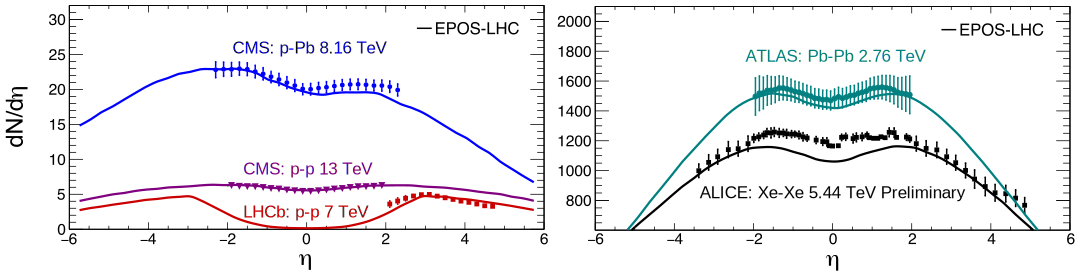
\includegraphics[width=\textwidth]{\main/beyond/fig/multiplicity_tuning_mod.pdf}
\caption{Comparison of charged particle multiplicity measurements at different center-of-mass energies and in different colliding systems with the EPOS-LHC model~\cite{Kim:2018ink}.}
\label{fig:multiplicity_tuning}
\end{figure}

Hadrons produced in the forward direction dominate the air shower development and experience significant nuclear modification\cite{Aaij:2017cqq}. The atmosphere consists of nitrogen and oxygen, therefore p-p collisions alone cannot constrain $\alpha$ and $\nmult$ to 5\,\%~\cite{dEnterria:2018kcz}. How to interpolate from p-p and p-Pb data to p-N or p-O is not clear, because the dominant nuclear effects for a light and heavy collision partner are expected to be different. Light nuclei are described by the shell model and nucleon correlations are important. Lead nuclei can be described by a simpler model, essentially a Wood-Saxon potential. The effect of correlations is reduced and cannot be probed well in experiments.
% Furthermore the collective effects which were not expected to be observed in light system (and as a consequence not implemented in specialized models for air shower simulation) seems to be very present in p-Pb~\cite{ALICE:2017jyt}.
The difficulty of predicting nuclear effects is demonstrated in Fig.~\ref{fig:multiplicity_tuning}, which shows EPOS-LHC predictions for Xe-Xe collisions, which deviate from the measurement, although EPOS-LHC provides a good description of p-p, p-Pb, and Pb-Pb data. The deviations in Xe-Xe are much larger than what is expected from a simple interpolation~\cite{Kim:2018ink}. Isolating peripheral p-Pb collisions to mimic p-O collisions with the same number of binary collisions is not a viable solution either, since this number is experimentally not well determined~\cite{Toia:2014wia}.

To achieve the desired accuracy and avoid systematic uncertainties, a direct measurement of multi-particle production of light hadrons in proton-oxygen collisions is highly desirable. The luminosity requirements to reach the physics goals are moderate. To reach a statistical accuracy of 5\,\%, 100\,M minimum-bias events are needed, which can be accumulated within a day of data-taking as described in Section~\ref{sec:pOrun}. The setup of p-O collisions would follow the successful rapid set-up procedure previously used in the 2012 p-Pb run and the 2017 Xe-Xe run.

\end{document}
